% Nejprve uvedeme tridu dokumentu s volbami
\documentclass[czech,bachelor]{diploma}
% Dalsi doplnujici baliky maker
\usepackage[autostyle=true,czech=quotes]{csquotes} % korektni sazba uvozovek, podpora pro balik biblatex
\usepackage[backend=biber, style=iso-numeric, alldates=iso]{biblatex} % bibliografie
\usepackage{dcolumn} % sloupce tabulky s ciselnymi hodnotami
%\usepackage{subfig} % makra pro "podobrazky" a "podtabulky"
\usepackage[cpp]{diplomalst}

\usepackage{amsmath}
\usepackage{amssymb}
\usepackage{tabularx}
\usepackage{booktabs} 
\usepackage{float}
\usepackage{tcolorbox}
\usepackage[edges]{forest}
\usepackage{xcolor}
\usepackage{listings}
\usepackage{graphicx}
\usepackage{subcaption}
\usepackage{pdflscape}
\usepackage{dirtree}

\newtcbox{\btboxround}{
  on line,
  colback=white,
  colframe=black,
  boxrule=0.5pt,
  arc=3pt,
  boxsep=0pt,
  left=2pt,
  right=2pt,
  top=2pt,
  bottom=2pt
}


% Zadame pozadovane vstupy pro generovani titulnich stran.
\ThesisAuthor{Roman Kratochvíl}

\ThesisSupervisor{Ing. Jakub Beránek}

\CzechThesisTitle{Využití behaviorálních stromů v Unreal Engine 5}

\EnglishThesisTitle{Impementing Behavioral Trees in Unreal Engine 5}

\SubmissionYear{2026}

\ThesisAssignmentFileName{ThesisAssignment.pdf}

% Pokud nechceme nikomu dekovat makro zapoznamkujeme.
\Acknowledgement{Rád bych na tomto místě poděkoval všem, kteří mi s prací pomohli, protože bez nich by tato práce nevznikla.}

\CzechAbstract{Tato bakalářská práce se zabývá využitím behaviorálních stromů pro implementaci chování nehrajících postav (NPC) v prostředí Unreal Engine 5 (UE5). Cílem práce je analyzovat principy behaviorálních stromů, porovnat je s jinými metodami implementace NPC a demonstrovat jejich praktické použití na vzorové hře. Práce se zaměřuje na návrh a realizaci netriviálního chování NPC, zahrnujícího například dynamickou interakci s prostředím, reakce na hráče a spolupráci mezi NPC. Součástí práce je dokumentace principů behaviorálních stromů, návrh několika typů chování, jejich implementace ve vzorové hře a využití verzovacího systému při vývoji.}

\CzechKeywords{behaviorální stromy, nehrající postavy, Unreal Engine 5, chování NPC, verzovací systém}

\EnglishAbstract{This bachelor’s thesis explores the use of behavioral trees for implementing non-player character (NPC) behavior within the Unreal Engine 5 (UE5) framework. The aim is to analyze the principles of behavioral trees, compare them with other NPC behavior implementation techniques, and demonstrate their practical application in a prototype game. The thesis focuses on designing and implementing complex NPC behaviors, including dynamic interaction with the environment, responses to player actions, and collaboration among NPCs. The work includes documentation of the principles of behavioral trees, the design of several behavior types, their implementation in a prototype game, and the use of a version control system during development.}

\EnglishKeywords{behavioral trees, non-player characters, Unreal Engine 5, NPC behavior, version control system}

\AddAcronym{UE5}{Unreal Engine 5}
\AddAcronym{NPC}{Non-playing character}

\addbibresource{sources.bib}

% Novy druh tabulkoveho sloupce, ve kterem jsou cisla zarovnana podle desetinne carky
\newcolumntype{d}[1]{D{,}{,}{#1}}


% Zacatek dokumentu
\begin{document}

% Nechame vysazet titulni strany.
\MakeTitlePages

% Jsou v praci obrazky? Pokud ano vysazime jejich seznam a odstrankujeme.
% Pokud ne smazeme nasledujici dve makra.
\listoffigures
\clearpage

% Jsou v praci tabulky? Pokud ano vysazime jejich seznam a odstrankujeme.
% Pokud ne smazeme nasledujici dve makra.
\listoftables
\clearpage

% A nasleduje text zaverecne prace.
\chapter{Úvod}

Herní vývojáři se snaží vytvářet herní prostředí, které působí pro hráče co nejvíce uvěřitelně a interaktivně. 
Jedním z hlavních prostředků, jak tohoto cíle dosáhnout, jsou nehráčské postavy.

Nehráčská postava (z anglického \textit{Non-Player Character}, dále zkráceně NPC) představuje herní entitu, 
která není přímo ovládána hráčem, ale jejíž chování je řízeno umělou inteligencí. NPC pomáhají řešit problém 
„mrtvého světa“, tedy prostředí, které nereaguje na hráčovy akce a neposkytuje odpovídající zpětnou vazbu.

S rostoucí komplexitou herních světů se zvyšují také nároky na chování NPC. Jednoduché skriptované reakce často 
nestačí k vytvoření realistického dojmu a mohou působit repetitivně nebo nepřirozeně. Návrh komplexního chování 
NPC proto představuje významný problém, který je nutné řešit vhodnými metodami umělé inteligence.

Jedním z přístupů k implementaci chování NPC jsou behaviorální stromy, které umožňují rozdělit rozhodovací logiku do přehledné hierarchické struktury. 
Tento přístup je v současnosti běžně využíván v herním vývoji díky své  modularitě a schopnosti reagovat na změny prostředí.

Tato práce se zaměřuje na využití behaviorálních stromů v prostředí Unreal Engine 5 (UE5), což je moderní herní 
engine poskytující nástroje pro tvorbu herní umělé inteligence. Cílem práce je analyzovat principy behaviorálních 
stromů a demonstrovat jejich využití při implementaci chování NPC ve vzorové hře.

\medskip

Struktura práce je následující. Kapitola~2 se zabývá principy behaviorálních stromů a jejich vlastnostmi. 
V kapitole~3 jsou popsány nástroje Unreal Engine~5, které slouží k implementaci chování NPC. 
Kapitola~4 představuje návrh a architekturu vytvořeného systému NPC. 
V kapitole~5 je popsána samotná implementace jednotlivých komponent. 
Kapitola~6 se věnuje testování a evaluaci vytvořeného řešení.
\chapter{Behaviorální stromy}

Tato kapitola popisuje základní principy behaviorálních stromů a jejich využití při návrhu chování NPC. 
Nejprve je vysvětleno, k čemu behaviorální stromy slouží a jakým způsobem se vykonávají. 
Poté jsou popsány základní typy uzlů, ze kterých se skládají. 
Závěr kapitoly shrnuje hlavní výhody a omezení tohoto přístupu s ohledem na návrh chování postav v UE5.

\section{Úloha behaviorálních stromů}

Behaviorální strom je způsob zápisu rozhodovací logiky autonomního agenta. 
V oblasti počítačových her se tímto agentem obvykle rozumí NPC, která na základě aktuální situace vybírá vhodné chování. 
Může například procházet herní prostředí, reagovat na hráče, komunikovat s jinou postavou nebo provádět interakce s objekty v herním prostředí.

Základní myšlenkou behaviorálního stromu je rozdělit chování na menší části. 
Místo jedné rozsáhlé podmínkové struktury je rozhodování popsáno pomocí uzlů uspořádaných do stromu. 
Některé uzly určují pořadí vyhodnocování, jiné ověřují podmínky a další vykonávají konkrétní akce. 
Díky tomu je možné složitější chování sestavit z jednodušších a lépe oddělených částí.\cite[s.~6]{colledanchise2018}

Tento způsob návrhu je vhodný zejména pro herní umělou inteligenci, protože chování postav musí být často reaktivní. 
Postava se nemůže rozhodnout pouze jednou a poté pokračovat bez ohledu na změny okolí. 
Naopak musí průběžně reagovat na pohyb hráče, změnu stavu objektů, dostupnost cesty nebo výsledek právě prováděné akce. 
Behaviorální strom umožňuje takové změny zachytit opakovaným vyhodnocováním rozhodovací logiky.\cite[s.~5]{colledanchise2018}

V této práci jsou behaviorální stromy důležité především proto, že představují hlavní prostředek pro řízení chování NPC v UE5. 
Pomocí nich lze jednotlivé typy chování oddělit do samostatných větví a následně určit, za jakých podmínek se mají spouštět.

\section{Základní princip vykonávání}

Behaviorální strom se vykonává od kořenového uzlu. 
Z něj je v pravidelných intervalech vysílán signál označovaný jako \textit{tick}. 
Tento signál postupuje stromem podle pravidel jednotlivých uzlů. 
Uzel je tedy vyhodnocen pouze tehdy, pokud k němu \textit{tick} dorazí.\cite[s.~6]{colledanchise2018}

Každý uzel po vyhodnocení vrací svému rodiči výsledek. 
V běžném pojetí behaviorálních stromů se používají tři základní návratové stavy. 
Stav \textit{Success} znamená, že uzel byl úspěšně dokončen. Stav \textit{Failure} vyjadřuje, že uzel nemohl svůj úkol splnit. 
Stav \textit{Running} se používá v případě, kdy akce stále probíhá a její výsledek zatím není známý.\cite[s.~9, tab.~1.1]{colledanchise2018}

Tyto návratové stavy tvoří základ komunikace mezi jednotlivými částmi stromu. 
Například akce přesunu na určité místo většinou nemůže skončit během jediného snímku hry. 
Dokud se postava pohybuje k cíli, uzel může vracet stav \textit{Running}. 
Jakmile je cíl dosažen, vrátí \textit{Success}. 
Pokud se cestu nepodaří najít, výsledek bude \textit{Failure}.

Opakované vyhodnocování stromu umožňuje postavě reagovat na aktuální stav hry. 
Pokud se například během pohybu změní podmínky v okolí, může být při dalším vyhodnocení zvolena jiná větev. 
Tím se behaviorální strom liší od jednoduchého skriptu, který pouze provede předem danou posloupnost příkazů bez průběžného přehodnocování situace.\cite[s.~9]{colledanchise2018}

\section{Struktura behaviorálního stromu}
Behaviorální strom je tvořen uzly, které jsou mezi sebou propojeny vztahem rodič--potomek. 
Výjimkou je kořenový uzel, který má vazby pouze na své potomky. 
Kořenový uzel stojí na začátku vyhodnocování a jednotlivé větve stromu popisují možné části chování.\cite[s.~6, kap.~1.3]{colledanchise2018}

Z pohledu struktury se uzly dělí do tří kategorií: kompozitní, dekorátorové a listové. 
Kompozitní uzly řídí tok vykonávání a určují, v jakém pořadí a za jakých podmínek se budou potomci vyhodnocovat. 
Dekorátorové uzly mají právě jednoho potomka a modifikují jeho chování nebo návratový stav. 
Listové uzly se nacházejí na koncích větví a představují buď podmínkové ověření stavu, nebo konkrétní akci. 
Podrobný popis každé kategorie je uveden v sekci \ref{sec:behavior_tree_node_types}.

Kompozitní uzly neurčují konkrétní akci ve světě hry, ale rozhodují o tom, která část stromu bude vyhodnocena. 
Typicky určují pořadí potomků nebo vybírají první větev, jejíž podmínky jsou splněny. 
Díky nim lze ve stromu vyjádřit například prioritu jednotlivých chování.

Podmínkové listové uzly slouží k ověření určitého stavu. 
V herním prostředí může jít například o kontrolu, zda postava vidí hráče, zda je v dosahu objekt, nebo jestli existuje platný cíl pohybu. 

Akční listové uzly představují samotné činnosti postavy. 
Mohou spustit pohyb, vybrat nový cíl, změnit hodnotu v \textit{Blackboard}, přehrát animaci nebo provést interakci s objektem. 
V UE5 jsou pro tyto části používány především uzly typu \textit{Task}.\cite[s.~76]{butler2023}

\section{Základní typy uzlů}
\label{sec:behavior_tree_node_types}

\subsection{Kompozitní uzly}

\textit{Kompozitní} uzly jsou řídicí uzly, které mají jednoho nebo více potomků. 
Jejich úlohou je určit, v jakém pořadí a za jakých podmínek se budou potomci vyhodnocovat. 
Mezi nejčastěji používané \textit{Kompozitní} uzly patří \textit{Sequence} a \textit{Selector} (v literatuře též zvaný jako \textit{Fallback}). 
V některých systémech se používá také uzel \textit{Parallel}.\cite[s.~6--7]{colledanchise2018}

\subsubsection{Sequence}

Uzel \textit{Sequence} slouží k postupnému vykonání několika kroků. 
Vyhodnocuje své potomky zleva doprava a pokračuje pouze tehdy, pokud předchozí potomek skončil úspěchem. 
Pokud některý potomek vrátí stav \textit{Failure}, selže celá sekvence. 
Pokud potomek vrátí \textit{Running}, znamená to, že daný krok ještě probíhá, a stejný stav vrací také celá sekvence.
Uzel \textit{Sequence} vrací návratovou hodnotu \textit{Success} pouze v tom případě, když všichni potomci tohoto uzlu mají návratovou hodnotu \textit{Success}.~\cite[s.~6]{colledanchise2018}

Tento uzel je vhodný pro chování, u kterého musí být splněno více kroků v přesném pořadí. 
Příkladem může být interakce NPC s předmětem. 
Postava nejprve ověří, zda je předmět dostupný, poté se k němu přesune a nakonec provede samotnou akci. 
Pokud už první podmínka není splněna, nemá smysl pokračovat v dalších krocích.

\subsubsection{Selector}

Uzel \textit{Selector} slouží k výběru první vhodné možnosti. 
Stejně jako \textit{Sequence} prochází své potomky zleva doprava, ale používá opačnou logiku. 
Jakmile některý potomek uspěje nebo stále probíhá, \textit{Selector} se zastaví a vrátí odpovídající stav. 
Selže pouze tehdy, když selžou všichni jeho potomci.~\cite[s.~7]{colledanchise2018}

\textit{Selector} se často používá pro vyjádření priorit. 
První větev může například popisovat reakci na hráče, druhá komunikaci s jinou postavou a třetí běžné pohybování po scéně. 
Strom se nejdříve pokusí vykonat chování s nejvyšší prioritou. 
Pokud pro něj nejsou splněny podmínky, pokračuje k další možnosti.

\subsubsection{Parallel}

Uzel \textit{Parallel} umožňuje vyhodnocovat více potomků současně.
Používá se v případech, kdy má agent provádět více činností najednou nebo kdy má během jedné akce průběžně sledovat další podmínku.
Chování uzlu je řízeno dvěma parametry: $N$ označuje celkový počet přímých potomků a $M$ je konfigurovatelný práh úspěchu ($1 \leq M \leq N$). 
Uzel vrátí stav \textit{Success}, pokud alespoň $M$ potomků uspěje, a stav \textit{Failure}, pokud více než $N - M$ potomků selže dříve, než je práh $M$ dosažen.\cite[s.~7]{colledanchise2018}

V UE5 existuje uzel \textit{Simple Parallel}. 
Ten umožňuje spustit hlavní úlohu a vedle ní vyhodnocovat další větev stromu.\cite[s.~76]{butler2023} 
Prakticky může jít například o~situaci, kdy se postava přesouvá k cíli a zároveň kontroluje, zda se nezměnil stav okolí.

\subsection{Dekorátorové uzly}
\label{subsec:decorators}

Dekorátorové uzly představují speciální typ řídicích uzlů, které mají právě jednoho potomka a slouží k úpravě jeho chování nebo návratového stavu.\cite[s.~8--9]{colledanchise2018}
Na rozdíl od ostatních řídicích uzlů, které určují tok vykonávání mezi více potomky, dekorátory modifikují výsledek nebo podmínky vykonání jediné podřízené větve.

V obecné teorii behaviorálních stromů mohou dekorátory například měnit návratové hodnoty uzlů (např. převrácení výsledku \textit{Success} na \textit{Failure}) 
nebo ovlivňovat způsob vykonávání, například omezením počtu opakování určité akce.\cite[s.~9]{colledanchise2018}

V prostředí UE5 mají dekorátory poněkud odlišnou vizuální strukturu. 
Jsou obvykle připojeny ke konkrétní větvi stromu a slouží především jako podmínky určující, zda může být daná větev vykonána.\cite[s.~93]{butler2023}
Nemají tedy vlastní samostatný vizuální uzel, jako tomu je u ostatních uzlů.
Typickým příkladem je kontrola hodnoty uložené v \textit{Blackboard}. 
Pokud je například dostupná reference na hráče, může se vykonat větev popisující reakci na hráče. 
V opačném případě je tato větev přeskočena a strom pokračuje jinou alternativou.

\subsection{Listové uzly}

Listové uzly se nacházejí na koncích větví behaviorálního stromu a nemají žádné potomky. 
Jejich úkolem je buď ověřit určitý stav, nebo provést konkrétní akci.\cite[s.~6]{colledanchise2018}

Podmínkové uzly kontrolují stav prostředí nebo interních dat postavy. 
Mohou například ověřit, zda je hráč v dosahu, zda je dostupný objekt pro interakci nebo zda postava již dokončila předchozí úkol. 
Výsledkem takového uzlu je zpravidla stav \textit{Success} nebo \textit{Failure}.\cite[s.~8]{colledanchise2018}
Stav \textit{Running} se u podmínkového uzlu nevyskytuje kvůli rozhodovací podstatě tohoto uzlu.

Akční uzly vykonávají konkrétní činnost. 
V UE5 se jedná zejména o uzly typu \textit{Task}. 
Ty mohou například spustit přesun pomocí navigačního systému, vybrat náhodný bod ve scéně, změnit hodnotu v \textit{Blackboard} 
nebo zavolat funkci implementovanou v \textit{Blueprint} či C++ třídě. 
Právě akční uzly propojují rozhodovací logiku behaviorálního stromu se skutečným chováním postavy ve hře.

Přehled návratových stavů všech popsaných typů uzlů je uveden v~tabulce~\ref{tab:BehaviorTreeNodeTypes}.

\begin{table}[H]
\centering
\small
\setlength{\fboxsep}{3pt}
\setlength{\fboxrule}{0.5pt}

\begin{tabularx}{\textwidth}{l c X X X}
\hline
\textbf{Typ uzlu} & \textbf{Symbol} & \textbf{Success} & \textbf{Failure} & \textbf{Running} \\
\hline
Selector & \fbox{?} & Pokud alespoň jeden potomek uspěje & Pokud všichni potomci selžou & Pokud alespoň jeden potomek vrátí Running \\
\hline
Sequence & \fbox{$\rightarrow$} & Pokud všichni potomci uspějí & Pokud alespoň jeden potomek selže & Pokud alespoň jeden potomek vrátí Running \\
\hline
Parallel & \fbox{$\rightrightarrows$} & Pokud $\geq M$~potomků uspěje & Pokud $> N - M$~potomků selže & V ostatních případech \\
\hline
Action & \fbox{text} & Po dokončení & Pokud nelze dokončit & Během provádění \\
\hline
Condition & \btboxround{text} & Pokud platí (true) & Pokud neplatí (false) & Nikdy \\
\hline
Decorator & $\diamond$ & Vlastní definice & Vlastní definice & Vlastní definice \\
\hline
\end{tabularx}

\caption{Typy uzlů v behaviorálním stromě.
Přeloženo podle~\cite[s.~9, tab.~1.1]{colledanchise2018}.}
\label{tab:BehaviorTreeNodeTypes}
\end{table}

Výše uvedená tabulka popisuje, jak fungují návratové hodnoty jednotlivých typů uzlů, ale neméně důležité je jejich vzájemné uspořádání ve stromě. 
Následující diagram ukazuje, jak lze popsané uzly kombinovat na konkrétním příkladu.

\begin{figure}[H]
\centering
\begin{forest}
  for tree={
    draw, rectangle, align=center, text centered,
    minimum width=3cm, minimum height=0.8cm,
    text width=2.8cm, font=\small,
    s sep=3mm, l sep=20mm,
    edge={-stealth}, anchor=north, inner sep=4pt,
  }
  [{ROOT}, fill=gray!30
    [{Selector~(?)}, fill=gray!15
      [{Sequence~($\rightarrow$)}, fill=gray!10
        [{Je hráč\\viditelný?},
            draw, rounded corners=6pt, align=center,
            text width=2.4cm, fill=orange!20]
        [{Uprav chování\\dle postupu\\hráče}]
      ]
      [{Sequence~($\rightarrow$)}, fill=gray!10
        [{Je v dosahu\\jiné NPC?},
            draw, rounded corners=6pt, align=center,
            text width=2.4cm, fill=orange!20]
        [{Zahaj komunikaci\\s~NPC}]
      ]
      [{Přesuň\\předmět}]
    ]
  ]
\end{forest}
\caption{Zjednodušená struktura behaviorálního stromu pro NPC.}
\label{fig:bt_npc_example}
\end{figure}

Obrázek~\ref{fig:bt_npc_example} znázorňuje, jak lze tři navrhovaná chování přirozeně uspořádat do jediného stromu. 
Uzel \textit{Selector} prochází větve zleva doprava a zkouší vždy chování s nejvyšší prioritou. 
Nejprve se pokusí o adaptaci vůči hráči. 
Podmínka viditelnosti hráče musí být splněna, aby se \textit{Sequence} vykonala.
Pokud hráč není viditelný, strom přejde na komunikaci s jiným NPC.
Není-li ani to možné, vykoná se výchozí chování, kterým je přesun předmětu. 
Tato větev nemá podmínku, takže k ní Selector vždy dojde. 
Uzel může skončit úspěchem i selháním podle toho, jak skončí daná akce.


\section{Výhody behaviorálních stromů}

Jednou z hlavních výhod behaviorálních stromů je modularita. 
Chování lze rozdělit do menších částí, které mají jasně určenou odpovědnost. 
Jedna větev může řešit pohyb, jiná reakci na hráče a další například komunikaci mezi postavami. 
Pokud jsou tyto části navrženy obecně, lze je později použít i v jiném chování nebo u jiné postavy.\cite[s.~38]{colledanchise2018}

Další výhodou je přehlednost. 
Stromová struktura umožňuje sledovat, jakým způsobem se postava rozhoduje. 
To je užitečné zejména v UE5, kde lze behaviorální strom vytvářet a upravovat v grafickém editoru. 
Vývojář tak nemusí procházet rozsáhlý zdrojový kód, ale může pracovat s vizuální reprezentací jednotlivých větví.\cite[s.~38]{colledanchise2018}

Důležitá je také reaktivita. 
Protože se strom vyhodnocuje opakovaně, může postava reagovat na změny prostředí. 
Pokud se například během běžného pohybu objeví hráč, může strom při dalším vyhodnocení přejít do větve s vyšší prioritou. 
Díky tomu chování nepůsobí pouze jako pevně připravená posloupnost příkazů, ale může se přizpůsobovat aktuální situaci.\cite[s.~38]{colledanchise2018}

Behaviorální stromy také podporují postupný vývoj. 
Na začátku může být strom jednoduchý a obsahovat pouze několik základních větví. 
Později lze přidávat další podmínky, akce a reakce, aniž by bylo nutné přepsat celý systém rozhodování. 
To je výhodné při vývoji herní umělé inteligence, protože chování postav se často upravuje podle výsledků testování.\cite[s.~38]{colledanchise2018}

\section{Omezení behaviorálních stromů}

Behaviorální stromy mají také určitá omezení. 
U rozsáhlých stromů může postupně klesat přehlednost, zejména pokud nejsou jednotlivé větve vhodně pojmenované nebo pokud se v nich opakuje podobná logika. 
V takovém případě může být obtížné zjistit, proč postava zvolila právě určité chování.

Dalším problémem může být špatně navržené pořadí větví. 
Uzel \textit{Selector} upřednostňuje potomky podle jejich pořadí. 
Pokud je důležitá větev umístěna příliš nízko, strom se k ní nemusí dostat, protože dříve uspěje jiná možnost. 
Chyba tedy nemusí být v samotné akci, ale ve struktuře rozhodování.

Behaviorální strom také vyžaduje průběžné vyhodnocování podmínek. 
U menšího počtu postav to obvykle nepředstavuje problém, ale u většího množství agentů nebo složitějších podmínek může být nutné řešit výkon. 
Při návrhu stromu je proto vhodné zvážit, které kontroly je nutné provádět často a které lze vyhodnocovat méně pravidelně.\cite[s.~42]{colledanchise2018}

\section{Srovnání s jinými technikami implementace chování NPC}

Behaviorální stromy nejsou ani zdaleka jedinou metodou řízení chování autonomních agentů.
V této sekci budou představeny a porovnány behaviorální stromy se dvěma alternativními přístupy, které jsou používány v~herním vývoji.
Jedná se o konečné automaty (\textit{FSM}) a~systémy založenými na hodnotě užitku (\textit{Utility-based system}).


\subsection{Konečné automaty}

Konečný automat (Finite State Machine, zkráceně FSM) je historicky nejrozšířenější přístup k~implementaci chování NPC. 
Agent se v~každém okamžiku nachází v~jednom z~předem definovaných stavů a~přechází mezi nimi na základě podmínek, které jsou průběžně vyhodnocovány.~\cite[s.~318]{millington2006}. 
Pro jednoduché NPC, kterému stačí pár stavů pro jeho věrohodnou implementaci chování, FSM bohatě stačí.
Asi nejlepším příkladem takových NPC jsou obecně zvířata.

Hlavním omezením FSM je škálovatelnost kvůli tomu, že s~rostoucím počtem stavů roste i~počet nutných přechodů mezi nimi. 
Každý nový stav tak může vyžadovat definování přechodů ze všech stavů ostatních. 
Tento jev je označován jako problém exploze stavů~\cite[s.~5]{colledanchise2018}. 
Další nevýhodou je obtížná znovupoužitelnost, protože chování navržené pro jednoho agenta 
lze jen těžko přenést na jiného agenta s~odlišnou sadou stavů.

V~kontextu implementovaného systému by použití FSM vedlo k~výraznému nárůstu počtu přechodů mezi stavy, zejména při kombinaci percepce, hlídkování 
a~interakcí s~objekty. 
Takový model by byl obtížně rozšiřitelný a~méně přehledný při ladění chování.

Behaviorální stromy tento problém řeší hierarchickým uspořádáním chování do větví. 
Dílčí chování jsou izolována do samostatných podstromů, které lze sdílet mezi různými agenty nebo opakovaně skládat do komplexnějšího chování. 
Přidání nového chování nevyžaduje úpravu existujících přechodů, ale pouze přidání nové větve do stromu. 
Z~těchto důvodů jsou behaviorální stromy považovány za přirozenou náhradu FSM v~situacích, kdy počet chování přesáhne několik málo stavů~\cite[s.~5]{colledanchise2018}.

\subsection{Systémy založené na hodnotě užitku}

Systémy založené na hodnotě užitku (utility-based systems) přiřazují každé
dostupné akci číselné skóre vyjadřující její vhodnost v~dané situaci. 
Agent nejčastěji vykoná akci s~nejvyšším skóre~\cite[s.~379]{millington2006}. 
Hodnota akce se typicky počítá jako vážená kombinace více faktorů. 
Například vzdálenosti od hráče, úrovně zdraví agenta nebo dostupnosti předmětů v~prostředí.

Výhodou tohoto přístupu je plynulý a~přirozený výběr chování. Agent nepřepíná diskrétně mezi stavy, ale průběžně reaguje 
na jemné změny situace. Pro simulace, kde je žádoucí, aby NPC působila organicky a~ne mechanicky předvídatelně, může být tato vlastnost přínosem.

Nevýhodou je obtížnost návrhu a~ladění. Správné nastavení vah a~hodnotících funkcí pro každou kombinaci faktorů vyžaduje opakované testování. 
Výsledné chování nevyplývá z~přehledné struktury, ale z~numerického výpočtu, jehož průběh je těžší sledovat a~opravovat.

V~případě implementovaného systému by bylo nutné definovat hodnotící funkce pro kombinaci 
více faktorů (např. vzdálenost hráče, slyšitelnost nebo dostupnost interakcí), což by výrazně zkomplikovalo ladění chování
bez zřejmého přínosu oproti explicitní hierarchii behaviorálního stromu.

Oproti tomu behaviorální strom dává návrháři explicitní kontrolu nad prioritou chování. 
Strukturou větví přímo určuje, co má přednost a za jakých podmínek, bez nutnosti kalibrovat numerické váhy.

\subsection{Zhodnocení}

Oproti FSM poskytují behaviorální stromy lepší škálovatelnost a~přehlednost při rostoucí komplexitě chování. 
Ve srovnání se systémy založenými na hodnotě užitku umožňují explicitní řízení priorit a~jednodušší ladění bez nutnosti 
definování numerických hodnotících funkcí.

Zvolený přístup se ukázal jako vhodný zejména pro implementaci hierarchického chování NPC, kde jednotlivé 
stavy (\texttt{Passive}, \texttt{Investigating}, \texttt{Attacking}) a~jejich přechody 
přirozeně odpovídají struktuře behaviorálního stromu.
\chapter{Unreal Engine 5 a AI systém}

Tato kapitola se zabývá nástroji Unreal Engine 5, které slouží k implementaci chování NPC. 
Nejprve je stručně vysvětlen pojem herního enginu a představen Unreal Engine 5. 
Následně jsou popsány konkrétní systémy, které jsou v této práci využity pro řízení chování postav.

\section{Herní engine a Unreal Engine 5}

Herní engine je softwarový nástroj, který poskytuje základní funkcionalitu potřebnou pro vývoj her. 
Typicky zahrnuje subsystémy pro vykreslování grafiky, fyzikální simulaci, práci se vstupy nebo správu herní logiky. 
Díky tomu se vývojář nemusí zabývat implementací těchto základních částí od začátku a může se soustředit na konkrétní obsah hry.\cite[s.~11--13]{gregory2018} 
Herní engine tedy pomáhá zvýšit potenciální produktivitu vývojáře.

Unreal Engine 5 (UE5) je moderní herní engine vyvíjený společností Epic Games. 
Kromě samotného běhu hry poskytuje také nástroje pro tvorbu herního obsahu a logiky. 
Jednou z jeho výhod je integrace systémů pro tvorbu umělé inteligence, které umožňují navrhovat chování NPC přímo 
v rámci enginu bez nutnosti použití externích knihoven.\cite{epic_gameplay_systems}

V UE5 je možné implementovat herní prvky a logiku buď pomocí C++, nebo pomocí proprietárního vizuálního skriptovacího systému, který se nazývá Blueprint.
V této práci jsou všechny systémy implementovány pomocí Blueprintu.


\section{Pawn a AI Controller}

V Unreal Engine 5 je objekt reprezentující postavu ve hře označován jako Pawn. 
Pawn určuje fyzickou přítomnost postavy ve scéně, například její polohu nebo pohyb.\cite{epic_pawn} 

Každý Pawn má controller, kterým je řízen. 
Pokud je postava ovládána hráčem, používá se Player Controller, v případě NPC pak AI Controller.\cite{epic_controller}

Typicky při převzetí kontroly nad Pawnem spouští behaviorální strom, který definuje jednotlivé akce NPC. 
Standardně platí mezi Pawn a Controller vazba 1:1, ale možná je i vícenásobná vazba (např. pro hry žánru RTS).
Propojení mezi AI Controllerem a Pawnem umožňuje controlleru ovládat pohyb i další aspekty chování postavy.

\section{Behaviorální strom v UE5}

Behaviorální strom je v Unreal Engine implementován jako samostatný asset, který lze upravovat pomocí grafického editoru.\cite{epic_bt} 
Princip jeho fungování odpovídá obecné teorii popsané v předchozí kapitole.

Strom se skládá z uzlů, které definují jednotlivé části chování. 
V UE5 se používají zejména tři typy uzlů:
\begin{itemize}
    \item \textit{Task} – představuje konkrétní akci (např. pohyb na cílovou pozici),
    \item \textit{Service} – pravidelně aktualizuje data během vykonávání větve,
    \item \textit{Decorator} – určuje podmínky, za kterých může být větev vykonána.
\end{itemize}

Behaviorální strom pracuje s daty uloženými v Blackboard a na jejich základě rozhoduje, jaká větev bude v daném okamžiku vykonána. 
Výhodou tohoto přístupu je přehlednost a možnost jednoduché úpravy chování bez zásahu do zdrojového kódu \cite[s.~80]{butler2023}.

\section{Blackboard}

Blackboard slouží jako sdílené datové úložiště pro behaviorální strom. 
Uchovává hodnoty přiřazené ke klíčům, například referenci na hráče, cílovou pozici nebo aktuální stav postavy.\cite{epic_bt} 

Samotný Blackboard neobsahuje žádnou logiku, pouze zpřístupňuje data ostatním částem systému. 
Tyto hodnoty mohou být nastavovány z různých míst, například z behaviorálního stromu nebo přímo z Blueprintu postavy.

\section{Navigační systém}

Pro pohyb NPC v prostředí využívá UE5 navigační systém založený na tzv. Navigation Mesh (NavMesh). 
NavMesh reprezentuje průchodné oblasti scény a určuje, kde se může postava pohybovat.\cite{epic_navsystem} 

Při vykonání akce pohybu (např. pomocí uzlu \textit{MoveTo}) je cílová pozice předána navigačnímu systému, který vypočítá cestu po NavMesh. 
Samotný pohyb postavy je následně realizován komponentou pro pohyb postavy.

\section{AI Perception}

AI Perception umožňuje NPC vnímat okolní prostředí prostřednictvím definovaných smyslů, například zraku nebo sluchu \cite{epic_perception}. 

Při zaznamenání podnětu (např. detekce hráče) dojde k vyvolání události, na jejímž základě se aktualizují hodnoty v Blackboardu. 
Behaviorální strom poté při dalším vyhodnocení reaguje na novou situaci a zvolí odpovídající chování.

\chapter{Návrh a architektura NPC systému}

Cílem této kapitoly je ukázat návrh architektury NPC v prostředí Unreal Engine~5, který využívá behaviorální stromy pro jeho řízení. 
Systém byl navržen tak, aby NPC dokázala reagovat na hráče, vnímat objekty v prostředí a v omezené míře spolupracovat s jinými NPC postavami.

V této práci bylo usilováno o dodržení oddělení odpovědností mezi jednotlivými funkčními částmi hry. 
Každá část systému má vymezenou roli: 
postava NPC zajišťuje fyzickou reprezentaci a provádění akcí, AI Controller zpracovává podněty z okolí 
a aktualizuje sdílenou paměť, behaviorální strom na základě těchto dat rozhoduje o aktuálním chování 
a Blackboard slouží jako datové úložiště propojující všechny části.

\section{Přehled systému a jeho komponent}

V projektu jsou vytvořeny dvě konkrétní NPC postavy, \texttt{BP\_Grandpa} a \texttt{BP\_Granny}, které sdílejí společnou rodičovskou třídu \texttt{BP\_NPC}. 
Tato bázová třída obsahuje veškerou herní logiku sdílenou všemi NPC: 
systém animací, správu zbraní, detekci interaktivních objektů v okolí a propojení s globálním stavem levelu. 
Konkrétní odvozené třídy slouží výhradně k odlišení vizuální podoby postav -- jiný skeletální mesh a animační blueprint. 
Přidání dalšího NPC do hry tak nevyžaduje duplikaci AI logiky.

AI logika je sdílena i na vyšší úrovni: obě postavy jsou řízeny stejným AI Controllerem \texttt{IAC\_NPC} a stejným behaviorálním stromem \texttt{BT\_NPC}. Každá instance NPC má přitom vlastní instanci Blackboardu \texttt{BB\_NPC}, takže jejich rozhodování je vzájemně nezávislé i přesto, že vychází ze stejné stromové definice.

Základní komponenty systému jsou:

\begin{itemize}
    \item \texttt{BP\_NPC} -- bázová třída NPC,
    \item \texttt{BP\_Grandpa}, \texttt{BP\_Granny} -- konkrétní NPC postavy,
    \item \texttt{IAC\_NPC} -- AI Controller,
    \item \texttt{BT\_NPC} -- behaviorální strom,
    \item \texttt{BB\_NPC} -- Blackboard,
    \item \texttt{BP\_RoutingManager} -- správce hlídkových tras,
    \item \texttt{BP\_PatrolRoute} -- reprezentace jednotlivé hlídkové trasy.
    \item \texttt{BPC\_InventorySystem} -- Systém inventáře, který využívají jak NPC, tak hráč
    \item \texttt{BPC\_InteractionSystem} -- Systém interakcí, který využívají jak NPC, tak hráč
\end{itemize}

Vzájemné závislosti mezi těmito komponentami jsou znázorněny na obrázku~\ref{fig:components}.

\begin{figure}[htbp]
    \centering
    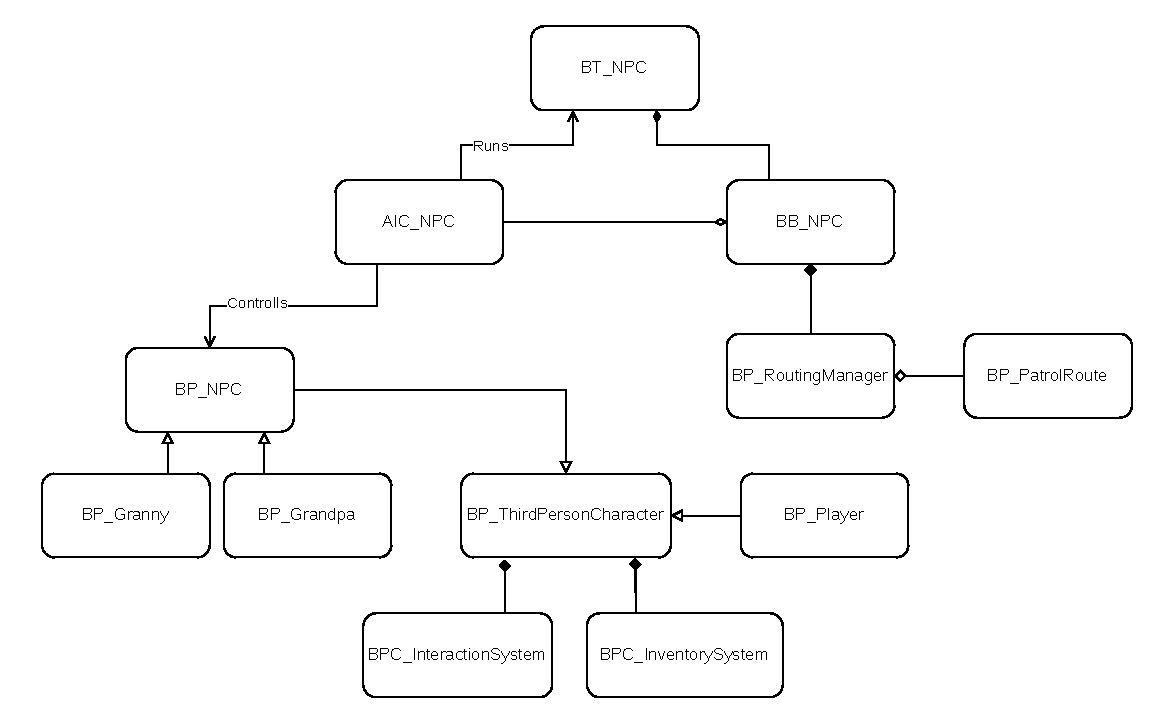
\includegraphics[width=\textwidth]{Figures/components.pdf}
    \caption{Přehled komponent systému NPC a jejich vzájemných vazeb}
    \label{fig:components}
\end{figure}

\section{Rozdělení odpovědností}

Návrh striktně odděluje rozhodování od vykonávání akcí. 
Toto oddělení je klíčovým principem využití behaviorálních stromů: 
strom rozhoduje, co má postava dělat, ale samotné provedení deleguje na třídu NPC.\cite[s.~178]{colledanchise2018}

Třída \texttt{BP\_NPC} implementuje konkrétní akce -- pohyb, útok, manipulaci se zbraní -- a neobsahuje žádnou rozhodovací logiku. 
Reaguje výhradně na příkazy vydané behaviorálním stromem prostřednictvím delegátů a custom eventů. 
Díky tomu lze rozhodovací logiku měnit nezávisle na fyzickém chování postavy.

AI Controller \texttt{IAC\_NPC} plní roli prostředníka mezi herním světem a behaviorálním stromem. 
Zpracovává podněty ze systému percepce, interpretuje je a přepisuje do odpovídajících klíčů Blackboardu. 
Controller sám nerozhoduje o chování NPC -- jeho úlohou je udržovat Blackboard aktuální tak, aby behaviorální strom mohl správně reagovat.

Behaviorální strom \texttt{BT\_NPC} je výhradním místem rozhodovací logiky. 
Na základě hodnot v Blackboardu vybírá odpovídající větev a prostřednictvím Tasků vydává příkazy k provedení konkrétních akcí.

\section{Stavový model NPC}

Chování NPC je strukturováno jako třístavový model. 
Každý stav odpovídá jedné hlavní větvi behaviorálního stromu a určuje, která část stromu bude vyhodnocována:

\begin{itemize}
    \item \textbf{Passive} -- NPC vykonává hlídkovou rutinu, pohybuje se po přidělené trase a příležitostně interaguje s prostředím nebo jinou NPC postavou,
    \item \textbf{Investigating} -- NPC prošetřuje podezřelý podnět, tedy detekovaný zvuk nebo pohyb sledovaného předmětu, na konkrétní souřadnici ve scéně,
    \item \textbf{Attacking} -- NPC reaguje na viděného hráče, vytasí zbraň a zahájí útok.
\end{itemize}

Přechody mezi stavy jsou výhradně v kompetenci AI Controlleru a jsou vyvolány událostmi ze systému percepce. 
Spatření hráče způsobí přechod do stavu \texttt{Attacking}, ztráta hráče ze zorného pole návrat do stavu \texttt{Passive} 
a detekce zvuku přechod do stavu \texttt{Investigating}. 
Aktuální stav je uložen v Blackboardu pod klíčem \texttt{State} jako hodnota výčtového typu \texttt{E\_AIState}. 
Schéma přechodů mezi stavy je znázorněno na obrázku~\ref{fig:state_model}.

\begin{figure}[H]
    \centering
    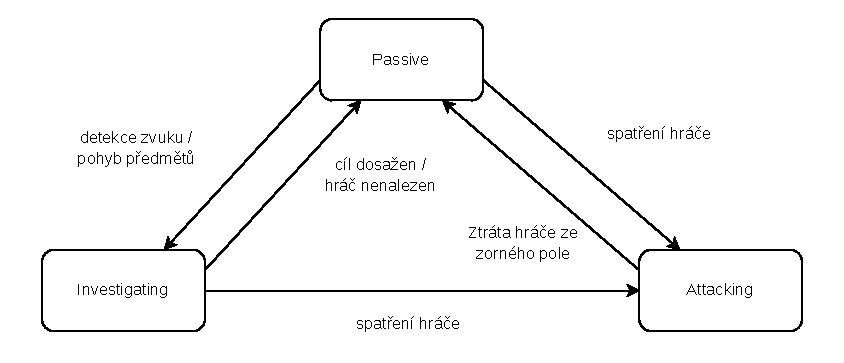
\includegraphics[width=\textwidth]{Figures/state_diagram.pdf}
    \caption{Přehled hlavních stavů NPC a přechodů mezi nimi}
    \label{fig:state_model}
\end{figure}

\section{Architektura behaviorálního stromu}

Behaviorální strom \texttt{BT\_NPC} je sdílen oběma NPC postavami. 
Každá postava spouští svou vlastní instanci stromu s vlastním Blackboardem, takže jejich rozhodování je nezávislé i při použití identické stromové struktury. 
Strom je spuštěn AI Controllerem při převzetí kontroly nad postavou, tedy při události \texttt{OnPossess}.

Na nejvyšší úrovni tvoří strom kořenový \texttt{Selector} se třemi větvemi. 
Každá větev je opatřena dekorátorem, který kontroluje hodnotu klíče \texttt{State} v Blackboardu. 
Selector prochází větve v pořadí od nejvyšší priority:

\begin{enumerate}
    \item \textbf{Attacking} (nejvyšší priorita) -- aktivní, pokud \texttt{State == Attacking},
    \item \textbf{Investigating} -- aktivní, pokud \texttt{State == Investigating},
    \item \textbf{Passive} (výchozí) -- aktivní, pokud \texttt{State == Passive}.
\end{enumerate}

Tato struktura zajišťuje, že útočné chování má vždy přednost před vyšetřováním a hlídkováním, čímž je implementována přirozená hierarchie priorit. 
Celý behaviorální strom je příliš obsáhlý na to, aby jej bylo možné zobrazit zde, a proto jej lze nalézt v příloze této práce~\ref{fig:bt_full}.

\subsection{Větev Passive}

Pasivní větev je nejkomplexnější částí stromu a implementuje hlídkovou rutinu NPC. 
Obsahuje jak Services, které běží periodicky na pozadí, tak Tasks vykonávané sekvenčně:

\begin{itemize}
    \item \texttt{BTS\_EnsurePatrolRoute} (Service) -- periodicky kontroluje, zda má NPC přiřazenou hlídkovou trasu; pokud ne, vyžádá ji od správce tras \texttt{BP\_RoutingManager},
    \item \texttt{BTT\_MakeRouteDecision} (Task) -- rozhoduje na základě aktuálního postupu po trase a náhodné hodnoty, zda NPC změní trasu,
    \item \texttt{BTT\_MoveAlongPatrolRoute} (Task) -- přesouvá NPC na další bod aktuální spline trasy,
    \item \texttt{BTT\_MakeInteractionDecision} (Task) -- rozhoduje, zda NPC interaguje s viděným objektem nebo s jinou NPC postavou; rozhodnutí závisí na typu interakce objektu a náhodné hodnotě \texttt{InteractionChance},
    \item \texttt{BTT\_GoToOtherNPC} (Task) -- naviguje NPC ke druhé NPC postavě,
    \item \texttt{BTT\_InteractWithOtherNPC} (Task) -- provede výměnu informací o pozicích předmětů mezi oběma NPC,
\end{itemize}

\subsection{Větev Attacking}

Útočná větev implementuje reakci na spatřeného hráče. 
Po přechodu do stavu \texttt{Attacking} větev nejprve zkontroluje, zda je zbraň vytasena, a pokud ne, spustí animaci vytasení. 
Poté nastaví AI focus na cíl, přepne NPC do běhu a zahájí útočnou animaci:

\begin{itemize}
    \item \texttt{BTDecorator\_IsWieldWeapon} (Decorator) -- podmínkově spustí vytasení zbraně pouze pokud ještě není vytasena,
    \item \texttt{BTT\_EquipWeapon} (Task) -- přehraje animaci vytasení zbraně,
    \item \texttt{BTT\_FocusTarget} (Task) -- nastaví rotační focus AI na cíl útoku uložený v Blackboardu pod klíčem \texttt{AttackTarget},
    \item \texttt{BTT\_SetMovementSpeed} (Task) -- přepne NPC do běhu nastavením maximální rychlosti pohybu,
    \item \texttt{BTT\_Attack} (Task) -- spustí útočnou animaci; dokončení animace je signalizováno zpět do Tasku prostřednictvím delegátu.
\end{itemize}

\subsection{Větev Investigating}

Vyšetřovací větev je nejjednodušší ze tří. NPC naviguje na souřadnici uloženou v Blackboardu pod klíčem \texttt{PointOfInterest}. 
Po dosažení cílové pozice, nebo pokud cíle nelze dosáhnout, stav automaticky přejde zpět do \texttt{Passive} a NPC pokračuje v hlídkování. 
Tato větev se aktivuje při detekci zvuku nebo při zjištění pohybu sledovaného předmětu.

\section{Tok dat v systému}

Tok informací v systému lze popsat jako sled kroků:

\begin{center}
\texttt{AI Perception} $\rightarrow$ \texttt{AI Controller} $\rightarrow$ \texttt{Blackboard} $\rightarrow$ \texttt{Behavior Tree} $\rightarrow$ akce NPC
\end{center}

AI Controller přijímá podněty ze systému percepce a přepisuje je do Blackboardu: aktualizuje stav NPC, ukládá pozici podezřelého místa nebo referenci na viděný objekt. Behaviorální strom při každém vyhodnocení přečte aktuální hodnoty z Blackboardu, vybere odpovídající větev a prostřednictvím Tasků vydá příkaz ke konkrétní akci. Samotnou akci pak vykoná třída \texttt{BP\_NPC}.

\section{Správa hlídkových tras}

Hlídkové trasy jsou reprezentovány třídou \texttt{BP\_PatrolRoute} jako spline-based křivky rozmístěné ve scéně. 
Pohyb po trase je obousměrný: NPC se pohybuje po bodech spline v jednom směru a po dosažení krajního bodu se otočí a vrátí se zpět po téže trase. 
Pro uzavřené smyčky je index bodu zabalován modulem délky trasy.

Přidělování tras jednotlivým NPC zajišťuje třída \texttt{BP\_RoutingManager}. 
Tento správce řeší problém kolize tras: zamezuje situaci, kdy by dvě NPC hlídkovaly na stejné trase a pohybovaly se synchronně. 
Při vyžádání nové trasy systém iteruje dostupné trasy v náhodně zamíchaném pořadí a přidělí první volnou. 
Obsazenost tras je evidována v interní mapě.

Součástí návrhu jsou tři sady tras odpovídající různým herním fázím (\texttt{Stage 1}, \texttt{Stage 2}, \texttt{Stage 3}). 
Příslušnost tras k dané fázi je určena tagem přiřazeným přímo instancím \texttt{BP\_PatrolRoute} ve scéně. 
Změna herní fáze tak přiřadí NPC jiné trasy bez jakékoliv modifikace behaviorálního stromu.

Variabilita chování je dále zajištěna pravděpodobnostním prvkem: každé NPC má při startu inicializovanou náhodnou hodnotu \texttt{RouteChangeChance} 
v rozsahu $0$--$1$, která určuje pravděpodobnost dobrovolné změny trasy po dosažení určitého úseku. 
Práh pro toto rozhodnutí je po každé změně rovněž randomizován v rozsahu $0{,}25$--$0{,}75$, takže NPC mění trasy nepravidelně a jejich pohyb nepůsobí mechanicky.

\section{Reprezentace znalostí NPC}

Chování NPC v této práci vyžaduje, aby postavy dokázaly pracovat s informacemi o objektech v herním prostředí. 
Nejedná se pouze o okamžitou reakci na podněty, ale také o schopnost zohlednit stav světa při rozhodování.

Znalosti NPC jsou reprezentovány kombinací globálního sdíleného stavu a lokálních dat jednotlivých postav.

\subsection{Globální stav objektů}

Informace o objektech ve scéně jsou spravovány centrálně pomocí třídy \texttt{BP\_GameStateBase}. 
Tato třída obsahuje registr sledovaných objektů, ve kterém jsou uloženy jejich referenční informace.

Každý objekt typu \texttt{BP\_BaseItem} se při inicializaci zaregistruje do tohoto registru a uloží svou výchozí pozici. 
Tato pozice představuje očekávaný stav objektu ve scéně.

Díky tomuto přístupu mají všechny NPC přístup ke konzistentní reprezentaci světa, aniž by bylo nutné 
udržovat redundantní kopie těchto dat pro každou postavu zvlášť.

\subsection{Lokální znalosti NPC}

Každá NPC si zároveň udržuje vlastní seznam známých objektů, který je uložen v její instanci. 
Tento seznam obsahuje reference na objekty, se kterými postava přišla do kontaktu nebo o nich získala informaci.

Lokální seznam slouží k:
\begin{itemize}
    \item uchování informací relevantních pro konkrétní NPC,
    \item vyhodnocování interakcí s objekty,
    \item rozhodování v rámci behaviorálního stromu.
\end{itemize}

Tato data nejsou sdílena přímo mezi NPC, ale každá postava je interpretuje samostatně na základě 
globálního stavu a vlastních zkušeností.

\subsection{Inicializace znalostí}

Při spuštění hry dojde k inicializaci registru objektů a jejich základních vlastností. 
NPC následně pracují s těmito daty během svého běžného chování, zejména v rámci pasivní větve behaviorálního stromu.

\subsection{Detekce změn v prostředí}

Změna stavu objektu je určena porovnáním jeho aktuální pozice s referenční hodnotou uloženou v globálním registru.

Pokud se tyto hodnoty liší, je objekt považován za přesunutý nebo chybějící. 
Tato informace je následně využita při rozhodování NPC, například pro přechod do stavu \textit{Investigating}.

Tímto způsobem je možné detekovat změny ve světě bez nutnosti složitějších mechanismů sledování historie.

\section{Komunikace mezi NPC}

Komunikace mezi NPC je realizována prostřednictvím Tasku \texttt{BTT\_InteractWithOtherNPC}, který se spouští v rámci pasivní větve behaviorálního stromu, když se dvě NPC dostatečně přiblíží. 
Mechanismus výměny informací probíhá ve třech krocích.

Nejprve aktivní NPC zjistí z globálního herního registru, tedy z \texttt{BP\_GameStateBase}, jaká je domácí neboli referenční pozice 
sledovaného předmětu -- tedy kde by měl předmět být. 
Poté přečte ze záznamu paměti druhé NPC, kde tento předmět druhá NPC naposledy viděla. 
Nakonec obě hodnoty porovná.

Pokud jsou pozice shodné, předmět nebyl přemístěn a NPC pokračují v hlídce. 
Pokud se pozice liší, byl předmět přemístěn hráčem. 
V takovém případě jsou u obou NPC nastaveny Blackboard klíče \texttt{LostItem?} na hodnotu \texttt{true} a \texttt{SearchShed} na hodnotu \texttt{true}, čímž jsou 
obě postavy instruovány k prohledání určitého místa. Zápis do Blackboardu druhého NPC probíhá přímým přístupem přes jeho AI Controller, bez použití centrálního 
koordinátora.

Jedná se o decentralizovaný mechanismus spolupráce: každé NPC si informace aktivně zjišťuje při každém setkání s partnerem 
a v případě nesouladu koordinovaně zahájí vyšetřování. 
Tím je naplněn požadavek na implementaci spolupráce mezi NPC postavami.

\section{Reakce na hráče a prostředí}

Reakce NPC na hráče je řízena systémem AI Perception implementovaným v AI Controlleru. 
Systém percepce pracuje se dvěma smysly: zrakem (\texttt{AISense\_Sight}) a sluchem (\texttt{AISense\_Hearing}).

Při zpracování vizuálních podnětů rozlišuje Controller tři scénáře. 
Pokud NPC spatří hráče, okamžitě přejde do stavu \texttt{Attacking} -- behaviorální strom při dalším vyhodnocení aktivuje útočnou větev s nejvyšší prioritou. 
Pokud hráč opustí zorné pole, NPC se vrátí do stavu \texttt{Passive}. 
Pokud NPC zaznamená interaktivní objekt ve scéně, uloží referenci na něj do Blackboardu pod klíč \texttt{SeenInteractible}, který pasivní větev stromu využije 
při rozhodování o interakci.

Zvukové podněty zpracovává Controller odděleně: pokud NPC uslyší zvuk a aktuálně není ve stavu \texttt{Attacking}, přejde do stavu \texttt{Investigating} 
s cílovou souřadnicí zdroje zvuku. 
Pokud NPC již útočí, zvuk je ignorován -- útok má vyšší prioritu a přechod do vyšetřovacího stavu by ho nežádoucně přerušil.

\section{Návrhová rozhodnutí}

Při návrhu systému byla přijata následující klíčová rozhodnutí:

\begin{itemize}
    \item \textbf{Společná bázová třída NPC} -- odděluje vizuální identitu od AI logiky a umožňuje přidávání nových typů NPC bez duplikace kódu. 
    Nová postava vyžaduje pouze nový mesh a animační blueprint.

    \item \textbf{Sdílený behaviorální strom s nezávislými Blackboardy} -- obě NPC sdílejí jednu definici stromu, ale každá rozhoduje na základě vlastních dat. 
    Tím je zajištěna konzistence chování při minimálním počtu assetů.

    \item \textbf{Oddělení rozhodování od vykonávání} -- AI Controller a behaviorální strom rozhodují, třída NPC vykonává. 
    Toto oddělení odpovídá doporučenému architektonickému vzoru pro využití behaviorálních stromů v Unreal Engine~5.

    \item \textbf{Blackboard jako centrální sdílená paměť} -- propojuje Controller, strom a Tasky bez přímých závislostí mezi nimi; každá část systému čte a zapisuje pouze do Blackboardu.

    \item \textbf{Pravděpodobnostní inicializace chování} -- náhodná inicializace hodnot \texttt{RouteChangeChance} a \texttt{InteractionChance} při startu 
    každého NPC zajišťuje, že i při sdíleném stromu se obě postavy chovají mírně odlišně a jejich pohyb nepůsobí synchronně.

    \item \textbf{Správce tras bez kolizí} -- \texttt{BP\_RoutingManager} zamezuje obsazení stejné trasy dvěma NPC současně, čímž zvyšuje přirozenost hlídkování 
    a zabraňuje vizuálně rušivé synchronizaci pohybu.
\end{itemize}


\chapter{Implementace systému NPC}
\label{sec:implementace}

Implementace byla rozdělena do několika navazujících částí. 
Nejprve je popsána realizace základní třídy NPC a jejích odvozených variant, poté implementace AI Controlleru, Blackboardu a behaviorálního stromu. 
Následující části se věnují konkrétním Taskům a Services, správě hlídkových tras, zpracování percepčních podnětů a komunikaci mezi NPC. 
Závěr kapitoly shrnuje vybraná implementační rozhodnutí a problémy, které bylo nutné při vývoji řešit. 

\section{Implementace BP\_NPC}
\label{sec:implementace-bp-npc}

Třída \texttt{BP\_NPC} je odvozena od třídy \texttt{BP\_ThirdPersonCharacter} a představuje základní implementaci všech nehráčských postav ve hře. 
Jejím hlavním účelem je realizace konkrétních akcí ve světě, zatímco rozhodovací logika je delegována na AI Controller a behaviorální strom. 
Třída tak slouží především jako vykonavatel příkazů generovaných vyššími vrstvami systému.

V rámci třídy jsou implementovány základní mechaniky pohybu, animací, útoku a interakcí s okolím. 
Aktualizace stavových proměnných souvisejících s pohybem probíhá periodicky v rámci události \texttt{Tick}, kde je z komponenty \texttt{CharacterMovement} získána aktuální rychlost postavy. 
Její velikost je následně ukládána do proměnné \texttt{Speed}, která slouží jako vstup pro animační systém. 
Současně je pomocí funkce \texttt{IsFalling} určováno, zda se postava nachází ve vzduchu, a výsledek je ukládán do proměnné \texttt{IsJumping}. 
Tyto proměnné umožňují animačnímu blueprintu plynule přepínat mezi jednotlivými animačními stavy.

Útočné chování je realizováno prostřednictvím vlastní události \texttt{Attack}, která je volána z behaviorálního stromu, k čemuž slouží \textit{task} \texttt{BTT\_Attack}. 
Po jejím spuštění je nastavena proměnná \texttt{IsAttacking} a přehrána odpovídající animační montáž pomocí uzlu \texttt{Play Montage}. 
Po dokončení nebo přerušení animace je proměnná \texttt{IsAttacking} opět resetována. 
Za povšimnutí stojí systém notifikací. V rámci animace (respektivě animační montáže) může vývojář vložit události na konkrétní snímky 
animace, čímž je mu dovoleno velmi flexibilně ovlivňovat dění v herním světě v průběhu animace.
Pro využití systému notifikací stačí vložit notifikaci na časové ose animace a zvolit buď jeden z předpřipravených 
událostí (např. \textit{Play Sound}), nebo vlastní událost, jak jde vidět na obrázku~\ref{fig:notify_timeline}.
Obrázek \ref{fig:notify_blueprint} poté ukazuje, jak taková událost může být implementována.
Tato konkrétní událost při zásahu hráče teleportuje hráče zpátky na \texttt{PlayerStart} (začátek levelu).

\begin{figure}[H]
    \centering

    \includegraphics[width=\textwidth]{Figures/AN_OnHitEvent.png}
    \caption{Umístění události \texttt{AN\_HitEvent} v animační montáži}
    \label{fig:notify_timeline}
\end{figure}

\begin{figure}[H]
    \centering

    \includegraphics[width=\textwidth]{Figures/AN_OnHitEventBlueprint.png}
    \caption{Implementace události \texttt{AN\_HitEvent} v blueprintu}
    \label{fig:notify_blueprint}
\end{figure}

Manipulace se zbraní je řešena pomocí dvojice událostí \texttt{EquipWeapon} a \texttt{UnequipWeapon}. 
Událost \texttt{EquipWeapon} přehrává animační montáž tasení zbraně a následně vytváří instanci zbraně pomocí \texttt{SpawnActor}. 
Vytvořený objekt je připojen ke kostře postavy na konkrétní socket. 
Reference na vytvořenou zbraň je uložena do proměnné \texttt{WeaponActor} a příznak \texttt{IsWieldingWeapon} indikuje, že postava aktuálně drží zbraň. 
Opačný proces je implementován v události \texttt{UnequipWeapon}, kde je zbraň odpojena a odstraněna.

Interakce s okolními objekty je realizována prostřednictvím kolizního systému. 
Při vstupu do kolize s objektem implementujícím rozhraní \texttt{BPI\_Interactible} je tato skutečnost detekována v události \texttt{OnComponentBeginOverlap}. 
Následně je získán AI Controller dané postavy a prostřednictvím jeho rozhraní je aktualizována odpovídající hodnota v Blackboardu, čímž je behaviorálnímu stromu signalizována možnost interakce. 
Při ukončení kolize (\texttt{OnComponentEndOverlap}) je tato informace opět odstraněna.

Třída dále obsahuje pomocnou funkci \texttt{SetMovementSpeed}, která na základě hodnoty výčtového typu nastavuje maximální rychlost pohybu postavy. 

Konkrétní postavy \texttt{BP\_Grandpa} a \texttt{BP\_Granny} dědí z třídy \texttt{BP\_NPC} a upravují především vizuální reprezentaci a animační parametry. 
Sdílená logika chování zůstává v třídě rodiče, čímž je minimalizována duplicita a zjednodušena případná rozšiřitelnost systému.

\section{Implementace AI Controlleru (IAC\_NPC)}
\label{sec:implementace-iac-npc}

Třída \texttt{IAC\_NPC}, odvozená od~\texttt{AIController}, představuje hlavní řídicí komponentu NPC. 
Jejím úkolem je zprostředkovat komunikaci mezi percepčním systémem, behaviorálním stromem a herním světem, a zároveň udržovat aktuální stav 
postavy prostřednictvím \textit{blackboardu}.

\subsection{Inicializace a napojení na behaviorální strom}

Po převzetí řízení nad postavou (událost \texttt{OnPossess}) dochází k inicializaci celého systému.
Nejprve jsou vyhledány všechny instance tříd reprezentujících hlídkové trasy a uloženy do interní kolekce.
Tento krok umožňuje dynamicky reagovat na změny ve scéně bez nutnosti pevného navázání tras v editoru.

Následně je spuštěn behaviorální strom \texttt{BT\_NPC}, přičemž před jeho spuštěním jsou do \textit{blackboardu}
zapsány výchozí hodnoty. Jedná se zejména o:
\begin{itemize}
    \item referenci na řízenou postavu (\texttt{SelfActor}),
    \item pravděpodobnost změny hlídkové trasy,
    \item pravděpodobnost interakce s objektem,
    \item počáteční hlídková trasa.
\end{itemize}

Inicializační fáze tak zajišťuje, že behaviorální strom pracuje nad konzistentní sadou dat a může okamžitě začít rozhodovací proces.

\subsection{Zpracování percepce}

Pro vytvoření dojmu smyslového vnímání u NPC se využívá komponenta \texttt{AIPerception}, která agreguje informace o okolních aktérech
a vyvolává událost \texttt{OnTargetPerceptionUpdated} při každé změně percepčního stavu.

Zpracování této události probíhá tak, že pro každý aktualizovaný aktér jsou získána
percepční data, jednotlivé podněty jsou analyzovány podle typu smyslu
a na základě výsledku jsou následně aktualizovány klíče v \textit{blackboardu}.

Pro rozlišení typu podnětu je využita pomocná metoda \texttt{CanSenseActor}, jejíž implementace 
je zobrazena na obrázku~\ref{fig:can_sense_actor}.
Metoda nejprve získá percepční data pro daného aktéra pomocí uzlu \texttt{Get Actors Perception}. 
Tato data jsou následně rozložena na jednotlivé stimuly, ze kterých se percepční informace skládá.

Následně je ověřeno, zda některý ze stimulů odpovídá požadovanému typu smyslu.

Pokud dojde ke shodě typů, metoda vrací informaci o úspěšném zaznamenání podnětu spolu s odpovídajícím stimulem. 
V opačném případě pokračuje vyhodnocování dalších stimulů, dokud není nalezen odpovídající podnět
nebo není seznam vyčerpán.

Pro obě NPC je nastaven zrak (\texttt{AISense\_Sight}) jako dominantní smysl.
Dominance vjemu znamená, že pokud je v rámci jedné aktualizace percepce
zaznamenáno více podnětů současně, je prioritně vyhodnocován právě tento smysl.

\begin{figure}[H]
    \centering

    \includegraphics[width=\textwidth]{Figures/CanSenseActor.png}
    \caption{Implementace metody CanSenseActor}
    \label{fig:can_sense_actor}
\end{figure}


\subsubsection{Zrakové podněty}

Zrakové podněty jsou zpracovávány funkcí \texttt{HandleSensedSight}, která navazuje na funkci \texttt{CanSenseActor}. 
Tato funkce přijímá referenci na detekovaného aktéra a hodnotu určující, zda byl aktér aktuálně úspěšně zaznamenán. 
Na rozdíl od sluchového podnětu zde nestačí pouze uložit polohu stimulu, protože zrak může detekovat různé typy objektů s odlišným významem pro chování NPC.

Prvním krokem je ověření, zda je detekovaným aktérem hráč. 
Pokud ano a podnět je úspěšně zaznamenán, funkce zjistí aktuální stav NPC pomocí \texttt{GetCurrentState}. 
Nenachází-li se NPC ve stavu \texttt{Attacking}, je zavolána funkce \texttt{SetStateAsAttacking}. 
Ta zapíše referenci na hráče do klíče \texttt{AttackTarget} a nastaví klíč \texttt{State} na hodnotu \texttt{Attacking}. 
Tím je behaviorálnímu stromu předána informace, že má přejít do větve útočného chování.

Druhou částí zpracování zrakového podnětu je práce s interaktivními objekty. 
Funkce ověřuje, zda detekovaný aktér implementuje rozhraní \texttt{BPI\_Interactible}. 
Pokud ano, je porovnán s hodnotou aktuálně uloženou v klíči \texttt{SeenInteractible}. 
V případě platného nově zaznamenaného objektu je reference na tento objekt uložena do \textit{blackboardu}. 
Pokud naopak NPC daný objekt již nezaznamenává a tento objekt odpovídá aktuálně uložené hodnotě, je klíč \texttt{SeenInteractible} vymazán.

Tato logika umožňuje, aby jeden percepční mechanismus sloužil jak pro reakci na hráče, tak pro průběžné sledování objektů, se kterými může NPC později interagovat. 
Rozhodnutí, zda s objektem skutečně interagovat, však není provedeno přímo v AI Controlleru, ale až v příslušné části behaviorálního stromu.


\subsubsection{Sluchové podněty}

Sluchové podněty jsou zpracovávány funkcí \texttt{HandleSensedSound}. 
Oproti zrakovým podnětům je tato část implementace jednodušší, protože zvukový podnět je reprezentován pouze polohou, nikoliv konkrétním cílovým aktérem.

Funkce nejprve zjistí aktuální stav NPC pomocí \texttt{GetCurrentState}. 
Pokud se postava nenachází ve stavu \texttt{Investigating}, je zavolána funkce \texttt{SetStateAsInvestigating}. 
Ta nastaví klíč \texttt{State} na hodnotu \texttt{Investigating} a uloží polohu zvukového podnětu do klíče \texttt{PointOfInterest}. 
Behaviorální strom tak při dalším vyhodnocení přejde do větve vyšetřování a NPC se přesune k místu, odkud byl podnět zaznamenán.

Pokud se NPC nachází ve stavu \texttt{Attacking}, ke změně na vyšetřovací stav nedochází. 
Tím je zajištěno, že zvukový podnět nepřeruší probíhající útočné chování.

\subsection{Správa stavů}

Aktuální stav NPC je reprezentován výčtovým typem \texttt{E\_AIState} a uložen v \textit{blackboardu}. 

Pro práci se stavem jsou implementovány pomocné metody:
\begin{itemize}
    \item \texttt{GetCurrentState} – vrací aktuální stav,
    \item \texttt{SetStateAsPassive} – nastaví pasivní chování,
    \item \texttt{SetStateAsAttacking} – nastaví útočný režim,
    \item \texttt{SetStateAsInvestigating} – nastaví režim vyšetřování.
\end{itemize}

Každá z těchto metod provádí nejen změnu stavu, ale i odpovídající aktualizaci dalších klíčů (např. cíle útoku nebo bodu zájmu).
Tím je zajištěno, že behaviorální strom vždy pracuje s konzistentními daty.

\subsection{Interakce s objekty}

Součástí implementace je i podpora interakcí s objekty ve scéně.
Při detekci aktéra, který implementuje rozhraní pro interakci, je jeho reference uložena do klíče \texttt{CurrentInteractionTarget}.
Pokud se jedná o nový objekt (odlišný od posledního), je tato změna propagována do \textit{blackboardu}.

Další metody umožňují reagovat na konkrétní události:
\begin{itemize}
    \item \texttt{NotifyItemPickUp} – zaznamená typ drženého objektu,
    \item \texttt{NotifyItemPlaced} – vymaže informaci o drženém objektu.
\end{itemize}

Tyto informace jsou následně využívány behaviorálním stromem pro rozhodování o dalším postupu.

\section{Implementace stromu chování (BT\_NPC)}
\label{sec:implementace-bt-npc}

Strom chování \texttt{BT\_NPC} se větví do tří hlavních větví (\texttt{Attacking}, \texttt{Investigating}, \texttt{Passive}).

Chování NPC je dále ovlivněno stavem několika klíčů v \textit{blackboard}, které reprezentují aktuální fázi hry.
Na základě těchto hodnot dochází ke změnám v dostupných hlídkových trasách.
\begin{itemize}
    \item \texttt{Fáze hledání} -- hráč hledá klíč od venkovní boudy,
    \item \texttt{Fáze pátrání} -- hráč odemknul venkovní boudu,
    \item \texttt{Fáze útěku} –- hráč se snaží utéct z pozemku.
\end{itemize}

Přechody mezi jednotlivými fázemi jsou řízeny pomocí \textit{blackboard klíčů} \texttt{SearchShed} a \texttt{IsShedOpen}, které odrážejí postup 
hráče ve hře.

Tato struktura přirozeně vyjadřuje prioritizaci chování: útok má přednost před~pátráním a~pátrání má přednost před~hlídkováním.
NPC zmenšují počet hlídkovacích tras, které si vybírají k hlídkování a zvyšují svůj pobyt venku, aby zamezili útěku hráče.

\subsection{Větev Attacking}

Větev \texttt{Attacking} reprezentuje chování NPC v situaci, kdy je detekován nepřítel.
Je aktivována na základě hodnoty klíče \texttt{State} v \textit{blackboardu}, který je nastaven na \texttt{Attacking}
v rámci zpracování percepčních podnětů.

V této větvi NPC využívá klíč \texttt{AttackTarget}, který obsahuje referenci na aktuální cíl.
Na základě této hodnoty dochází k pohybu směrem k cíli a následnému provedení útoku.

Samotný útok je realizován pomocí úlohy \texttt{BTT\_Attack}, která spouští odpovídající animační montáž (viz \ref{fig:notify_timeline}) a řídí průběh útočné akce.

Chování v této větvi má nejvyšší prioritu, což znamená, že při detekci nepřítele dochází k okamžitému přepnutí z ostatních stavů do útočného režimu.

\subsection{Větev Investigating}

Větev \texttt{Investigating} reprezentuje chování NPC při vyhodnocení podezřelého podnětu,
typicky na základě sluchového vjemu.

Aktivace této větve je řízena hodnotou klíče \texttt{State} v \textit{blackboard},
který je nastaven na \texttt{Investigating} ve funkci \texttt{HandleSensedSound}.
Současně je do klíče \texttt{PointOfInterest} uložena poloha, odkud byl podnět zaznamenán.

V rámci této větve se NPC přesouvá k uložené pozici a provádí její prohledání.
Konkrétní průběh tohoto chování je řízen behaviorálním stromem na základě hodnoty klíče \texttt{PointOfInterest}.

Pokud během vyšetřování dojde k detekci nepřítele, dochází ke změně stavu na \texttt{Attacking}, což má vyšší prioritu a způsobí opuštění této větve.
Pokud se naopak ukáže, že prozkoumávané místo není ničím důležité, tak dojde ke změně do stavu \texttt{Passive}.

\subsection{Větev Passive}

Větev \texttt{Passive} reprezentuje výchozí chování NPC v situaci, kdy není detekován žádný významný podnět.
Slouží jako základní režim, ve kterém NPC vykonává hlídkování.

V rámci této větve je využita služba \texttt{BTS\_EnsurePatrolRoute}, která zajišťuje, že má NPC přiřazenou platnou hlídkovou trasu.
V případě, že žádná trasa není nastavena, služba vyžádá její přidělení prostřednictvím systému \texttt{BP\_RoutingManager}.

Samotný pohyb po trase je realizován úlohou \texttt{BTT\_MoveAlongPatrolRoute}, která postupně naviguje NPC mezi jednotlivými body hlídkové trasy.

Taktéž v této větvi probíhají interakce \texttt{BTT\_InteractWithActor}, přemisťování předmětů \texttt{BTT\_PlaceItem}, komunikace 
s jiným NPC \texttt{BTT\_InteractWithOtherNPC} a dělání rozhodnutí o změnách hlídkových tras. 

Pokud NPC nemá k dispozici žádnou trasu, setrvává na místě do doby, než je jí trasa přidělena.
Tato větev tak zajišťuje kontinuální chování NPC i v případě absence dalších podnětů z okolí.

\section{Implementace úloh a služeb}
\label{sec:implementace-tasky}

Tato část popisuje vybrané úlohy a služby behaviorálního stromu, které přímo propojují rozhodovací logiku stromu s konkrétními akcemi NPC ve světě hry. 
Úlohy typu \textit{Task} slouží k provedení jednorázové nebo déle trvající akce, zatímco služby typu \textit{Service} průběžně aktualizují data potřebná pro vykonávání dané větve stromu.

\subsection{BTT\_Attack}

Úloha \texttt{BTT\_Attack} realizuje spuštění útoku řízené NPC postavy. 
Při vykonání úlohy je nejprve získána reference na ovládanou postavu a ta je přetypována na \texttt{BP\_NPC}. 
Následně je na této postavě zavolána událost \texttt{Attack}, která je implementována v třídě \texttt{BP\_NPC} a zajišťuje přehrání útočné animační montáže.

Úloha není ukončena okamžitě po spuštění animace. 
Místo toho se naváže na událost \texttt{OnAttackEnd}, která je vyvolána až po dokončení útoku. 
Teprve poté je zavoláno \texttt{Finish Execute} s výsledkem \texttt{Success}. 
Tím je zajištěno, že behaviorální strom pokračuje až ve chvíli, kdy je útočná akce skutečně dokončena.

Součástí úlohy je také obsluha přerušení. 
Pokud je úloha předčasně ukončena, například kvůli přechodu do jiné větve stromu, je zastaven pohyb controlleru, zrušen aktuální focus 
a úloha je ukončena pomocí \texttt{Finish Abort}. 
Tento postup zabraňuje tomu, aby NPC po přerušení útoku pokračovalo v neaktuální akci.

\subsection{BTT\_MoveAlongPatrolRoute}

Úloha \texttt{BTT\_MoveAlongPatrolRoute} zajišťuje pohyb NPC po aktuálně přiřazené hlídkové trase. 
Při spuštění úloha načte z \textit{blackboardu} hodnotu klíče \texttt{CurrentPatrolRoute} a zkontroluje se, zda je klíč platný.

Z trasy je následně získána světová pozice aktuálního bodu pomocí funkce \texttt{GetSplinePointAsWorldPosition}. 
Na tuto pozici je NPC navigována pomocí uzlu \texttt{AI MoveTo}. 
Po úspěšném dosažení cíle je na trase zavolána funkce \texttt{IncrementPatrolRoute}, která posune interní ukazatel na další bod trasy. 
Poté je úloha ukončena pomocí \texttt{Finish Execute} s výsledkem \texttt{Success}.

Pokud se nepodaří získat platnou trasu, přetypování selže nebo pohyb k cílové pozici není úspěšný, úloha je ukončena neúspěšně. 
Součástí implementace je také reakce na přerušení úlohy, při které je pohyb NPC zastaven a úloha je ukončena pomocí \texttt{Finish Abort}.

\subsection{BTS\_EnsurePatrolRoute}

Služba \texttt{BTS\_EnsurePatrolRoute} zajišťuje, že má NPC během pasivního chování přiřazenou platnou hlídkovou trasu. 
Při aktivaci služby je z \textit{blackboardu} načten klíč \texttt{CurrentPatrolRoute}. 
Pokud je tato hodnota již nastavena, není nutné trasu měnit.

V případě, že NPC platnou trasu nemá, služba načte z \textit{blackboardu} referenci na systém \texttt{BP\_RoutingManager}. 
Po ověření platnosti této reference je řízená postava přetypována na \texttt{BP\_NPC} a je zavolána funkce \texttt{ChangeRoute}. 
Výsledkem této funkce je nová hlídková trasa, která je následně uložena zpět do klíče \texttt{CurrentPatrolRoute}.

Tato služba odděluje samotné přidělování tras od úlohy, která po trase pouze vykonává pohyb. 
Díky tomu může být logika výběru trasy spravována centralizovaně v \texttt{BP\_RoutingManager}, zatímco behaviorální strom pracuje pouze 
s aktuálně přiřazenou trasou.

\section{Implementace hlídkových tras}
\label{sec:implementace-routing}

\subsection{BP\_PatrolRoute}

Třída \texttt{BP\_PatrolRoute} reprezentuje hlídkovou trasu pomocí komponenty typu \texttt{SplineComponent}, která definuje plynulou křivku 
ve~světovém prostoru herní úrovně. 
Jednotlivé hlídkové body nejsou explicitně reprezentovány samostatnými komponentami, ale odpovídají bodům spline křivky.

Pro práci s~trasou třída poskytuje několik metod. 
Metoda \texttt{GetSplinePointAsWorldPosition} vrací světovou polohu bodu spline se zadaným indexem.
Dále je implementována metoda \texttt{IncrementPatrolRoute}, která aktualizuje index aktuálního bodu na základě směru pohybu a typu trasy.

Trasa může být buď cyklická, nebo otevřená. 
V případě cyklické trasy je index inkrementován o modulo počtu bodů křivky.
U otevřené trasy dochází při dosažení koncových bodů ke změně směru průchodu (tzv. ``ping-pong'' pohyb), což je realizováno přepínáním hodnoty 
proměnné \texttt{Direction}.

Pomocné metody \texttt{GetRouteProgress} a \texttt{GetRouteType}
umožňují získat relativní postup po trase a určit, zda se jedná
o cyklickou či necyklickou trasu.

\subsection{BP\_RoutingManager}

Třída \texttt{BP\_RoutingManager} implementuje správu hlídkových
tras a jejich přidělování NPC postavám.

Při inicializaci v rámci události \texttt{BeginPlay} jsou vyhledány všechny dostupné 
hlídkové trasy v levelu a ty jsou uloženy do interních kolekcí.
Trasy jsou dále rozděleny do skupin na základě tagů aktérů (např. \texttt{STAGE2}, \texttt{STAGE3}), což umožňuje řídit, které trasy jsou dostupné 
v různých fázích hry.

Obsazenost tras není reprezentována přímo v objektech tras, ale je evidována v mapě \texttt{Occupants}, která mapuje instance NPC na jim přidělené trasy.

Metoda \texttt{AcquireRoute(Requester)} vrací trasu pro daného žadatele. 
Pokud již má NPC trasu přidělenou, je vrácena tato existující trasa. 
V opačném případě dojde k náhodnému promíchání seznamu tras a následně k výběru první neobsazené trasy.
Vybraná trasa je zapsána do mapy \texttt{Occupants}.

Metoda \texttt{IsRouteOccupied(Route)} ověřuje, zda je daná trasa aktuálně obsazena některou NPC postavou.

Metoda \texttt{ReleaseRoute(Requester)} odstraní záznam o přiřazení trasy danému NPC a tím ji uvolní pro další použití.

Metoda \texttt{ChangeRoute(Requester)} nejprve uvolní aktuální trasu a následně přidělí novou trasu pomocí \texttt{AcquireRoute}.
Specifické varianty \texttt{ChangeRoute\_Stage2} a \texttt{ChangeRoute\_Stage3} vybírají trasu pouze z příslušné podmnožiny tras definované tagy.

Pokud není žádná volná trasa k dispozici, metoda vrací hodnotu \texttt{None}, přičemž NPC může o přiřazení požádat znovu v dalším průchodu stromem.

\section{Sdílení informací o předmětech}
\label{sec:sharing_information}

Komunikace mezi NPC není v implementaci řešena přímým předáváním informací o detekovaných hrozbách. 
Namísto toho je zaměřena na sdílení znalostí o herních předmětech, především o jejich výchozích pozicích a případném nesprávném umístění.

Základním prvkem tohoto systému je třída \texttt{BP\_GameStateBase}, která udržuje společný seznam předmětů ve scéně. Každý předmět odvozený
od třídy \texttt{BP\_BaseItem} se při spuštění zaregistruje do tohoto seznamu pomocí funkce \texttt{AddToItemList}. 
Současně je uložena jeho výchozí poloha prostřednictvím funkce \texttt{SetItemHomePosition}.
Tím vzniká sdílený zdroj informací, ke kterému mohou NPC při svém chování přistupovat.

Pro zjištění předmětu, který je potřeba uklidit, slouží funkce \texttt{RequestItemCleanup}. 
Ta prochází registrované předměty a hledá takový, který je označen jako nesprávně umístěný. 
Pokud je takový předmět nalezen, vrací referenci na něj společně s jeho aktuální polohou.

Vlastní výměna informací mezi NPC je realizována v úloze \texttt{BTT\_InteractWithOtherNPC}. 
Tato úloha vyhledá ostatní instance \texttt{BP\_NPC} ve scéně a vybere jinou postavu než tu, která úlohu právě vykonává. 
Následně pracuje se seznamy známých předmětů jednotlivých NPC a porovnává informace o jejich umístění.

Pokud NPC získá od jiné postavy relevantní informaci o předmětu, může tuto informaci využít pro aktualizaci vlastních hodnot v \textit{blackboardu}. 
V implementaci se tímto způsobem pracuje například s informací o ztraceném předmětu a s klíči souvisejícími s hledáním boudy. 
Díky tomu mohou NPC nepřímo sdílet informace o stavu herního světa, aniž by mezi nimi existoval samostatný systém zpráv nebo událostí.

\section{Implementační problémy a rozhodnutí}
\label{sec:problems_and_solutions}
Původní návrh systému komunikace mezi NPC počítal s individuální komponentou \texttt{BPC\_MemorySystem} připojenou ke každé NPC postavě. 
Tato komponenta měla uchovávat záznamy o objektech, se kterými postava přišla do kontaktu, a umožňovat přímou výměnu těchto záznamů mezi NPC.

Při implementaci se však ukázalo, že synchronizace paměťových záznamů mezi instancemi komponent napříč různými postavami nebyla spolehlivá. 
Docházelo k nekonzistentním stavům, kdy si NPC předávaly neaktuální nebo neplatné reference.

Problém byl vyřešen přechodem na centralizovaný přístup prostřednictvím třídy \texttt{BP\_GameStateBase}. 
Místo individuálních paměťových komponent byl zaveden společný registr objektů dostupný všem NPC. 
Každý objekt si při inicializaci zaregistruje výchozí polohu, ke které NPC přistupují při rozhodování. 
Přímá výměna paměťových záznamů byla nahrazena porovnáním lokálního seznamu \texttt{ItemsKnownList} s tímto centrálním registrem.




\chapter{Testování a evaluace řešení}
\label{sec:testing}

Testování systému NPC probíhalo manuálně v rámci herní scény. 
Cílem testování bylo ověřit, zda implementovaná chování odpovídá návrhu a zda jednotlivé mechanismy fungují v očekávaných situacích.

\begin{table}[H]
\centering
\begin{tabular}{|p{0.28\textwidth}|p{0.42\textwidth}|p{0.18\textwidth}|}
\hline
\textbf{Scénář} & \textbf{Očekávané chování} & \textbf{Výsledek} \\
\hline
Přechody mezi stavy & NPC přechází mezi stavy \texttt{Passive}, \texttt{Investigating} a \texttt{Attacking}. & Ověřeno \\
\hline
Zraková percepce & Detekce hráče vede k přechodu do stavu \texttt{Attacking}. & Ověřeno \\
\hline
Ztráta vizuálního kontaktu & NPC se po ztrátě cíle vrací do pasivního chování. & Ověřeno \\
\hline
Sluchová percepce & Zvukový podnět vede k přechodu do stavu \texttt{Investigating}. & Ověřeno \\
\hline
Hlídkování NPC & NPC se pohybuje po přiřazené hlídkové trase. & Ověřeno \\
\hline
Změna hlídkové trasy & NPC po splnění podmínek změní aktuální trasu. & Ověřeno \\
\hline
Fázově řízené trasy & NPC upravují výběr tras podle fáze hry. & Ověřeno \\
\hline
Interakce s objekty & NPC dokáže interagovat s objekty (např. otevírání dveří). & Ověřeno \\
\hline
Sebrání předmětu & NPC dokáže sebrat interaktivní předmět (např. klíč). & Ověřeno \\
\hline
Položení předmětu & NPC po sebrání přesune předmět na jiné místo. & Ověřeno \\
\hline
Sdílení informací & NPC si předávají informace o předmětech. & Neověřeno \\
\hline
\end{tabular}
\caption{Přehled manuálně ověřených scénářů}
\label{tab:testovaci-scenare}
\end{table}

Z tabulky~\ref{tab:testovaci-scenare} vyplývá, že základní mechanismy systému fungují dle očekávání. 
Byla ověřena zejména správná funkce percepce, přechodů mezi stavy a hlídkovacího chování NPC.

Naopak některé pokročilejší části systému nebyly v rámci testování spolehlivě ověřeny. 
Konkrétně se jedná o manipulaci s předměty po jejich sebrání a sdílení informací mezi NPC. 
Tyto části proto nelze považovat za plně otestované a představují omezení aktuální implementace.
\chapter{Závěr}
\label{sec:conclusion}

Cílem této bakalářské práce bylo navrhnout a implementovat systém
chování nehráčských postav (NPC) v herním prostředí s využitím
behaviorálních stromů v prostředí Unreal Engine~5.

Navržený systém kombinuje využití \texttt{AI Controlleru},
\texttt{Blackboardu} a behaviorálního stromu, což umožňuje
modulární a přehlednou implementaci jednotlivých typů chování.
Součástí řešení je také systém percepce založený na zrakových
a sluchových podnětech a mechanismus sdílení informací o
předmětech prostřednictvím \texttt{GameState}.

V rámci implementace se podařilo vytvořit funkční prototyp,
ve kterém NPC dokáží hlídkovat, reagovat na hráče,
interagovat s objekty ve scéně a pracovat s předměty.
Chování jednotlivých postav odpovídá návrhu a je snadno
rozšiřitelné o další prvky.

Testování ukázalo, že základní mechanismy systému fungují
spolehlivě, zejména v oblasti percepce, přechodů mezi stavy
a pohybu po hlídkových trasách. Naopak některé pokročilejší
části, jako manipulace s předměty nebo sdílení informací mezi
NPC, nebyly plně ověřeny a představují prostor pro další
vylepšení.

\section{Možná rozšíření a budoucí práce}

Navržený systém chování NPC by bylo možné dále rozšířit o reakce na dynamické změny prostředí. 
Jednou z možností je zohlednění denní doby a povětrnostních podmínek.
Například v nočních hodinách by NPC mohly trávit více času v interiéru, zatímco během dne by se častěji pohybovaly v okolí domu. 
Podobně by bylo možné simulovat vliv deště, který by negativně ovlivňoval percepční schopnosti NPC, například zhoršením sluchu.

Dalším rozšířením by bylo zavedení interaktivních prvků v prostředí, jako jsou například světelné vypínače.
NPC by mohly reagovat na změny osvětlení v místnostech, například snahou rozsvítit při vstupu do tmavého prostoru, nebo naopak vyhýbáním se neosvětleným místnostem.
Takové chování by mohlo přispět k vyšší věrohodnosti a variabilitě simulace.

Uvedená rozšíření nebyla v rámci této práce implementována, je ale možné takových cílů dosáhnout při dalším vývoji této hry.

\endinput


% Seznam literatury
\printbibliography[title={Literatura}, heading=bibintoc]

% Prilohy
\appendix
\begin{sidewaysfigure}
    \centering
    \includegraphics[width=\textheight, keepaspectratio]{Figures/behavior_tree.png}
    \caption{Kompletní struktura behaviorálního stromu použitého v systému NPC}
    \label{fig:bt_full}
\end{sidewaysfigure}
\chapter{Struktura projektu}

Projekt byl verzován pomocí verzovacího systému Git. 

Repozitář je dostupný online na adrese \url{https://github.com/bad-account/bachelor_thesis}.

\dirtree{%
.1 /.
.2 BachelorThesis\DTcomment{LaTeX projekt}.
.3 BachelorThesis.pdf\DTcomment{PDF soubor s textem práce}.
.2 Config\DTcomment{konfigurace projektu}.
.2 Content\DTcomment{herní assety}.
.2 videos\DTcomment{záznamy z testování}.
.2 Descent\_into\_Despair.uproject\DTcomment{Unreal Engine Project File}.
.2 README.md\DTcomment{popis repozitáře}.
}




% Priloha vlozena primo do hlavniho LaTeX souboru. Ne vsechny prilohy je nutne mit ve zvlastnich souborech.
%\chapter{Dlouhý zdrojový kód}
%\lstinputlisting[label=src:CppExternal,caption={Dlouhý zdrojový kód v jazyce C++ načtený s externího %souboru}]{SourceCodes/ArraySortingAlgorithms.cpp}

\end{document}
